% Drawing 144/07-8 -- folder 144, batch 07, archive page 135 (PDF page 136).
% Transcription: une variante du cube précédent ($\Pi' = \mathfrak{S}^!$, $\mathcal{M}^!$, $\mathcal{M}$, $\mathcal{M}^{+!}$, $\mathcal{M}^+$, $\mathfrak{S}^{+!}\Rightarrow\mathfrak{S}^+$), couverte de boucles qui la cancellent.
% Kind: variant of the cube, cancelled by loops. Method 2 (schematic redraw from the facsimile). Status: partial.
% Notes: The cube Pi' = S^!, M^!, M, M^{+!}, M^+, S^{+!} => S^+ (the last a double arrow on the page, drawn single), overrun by long thin loops that cancel it; the loops are drawn struck, three of them, approximately. The other diagrams on the page (II above, III below) have no mark of their own here and are not drawn. Which strokes are arrows is a reading under the loops.
% Coordinates: 1 unit = 1 mm = 1/100 of the crop width (bbox in page fractions: [0.22, 0.27, 0.59, 0.43]).
% Redrawn by Claude (claude-opus-5-5), issue #73, 2026-11-07; not checked by a human; not compiled (no TeX in the session).
% Rights: reproduces part of the work -- behind RENDER_TRANSCRIPTS, never published by itself.
\documentclass[tikz,border=3pt]{standalone}
\usepackage{amsmath,amssymb}
\usetikzlibrary{patterns,arrows.meta}
\tikzset{pencil/.style={black!45}, struck/.style={black!35}, mark/.style={circle,draw,inner sep=1.3pt}, pt/.style={circle,fill,inner sep=0.9pt}, opt/.style={circle,draw,fill=white,inner sep=1.1pt}}
\begin{document}
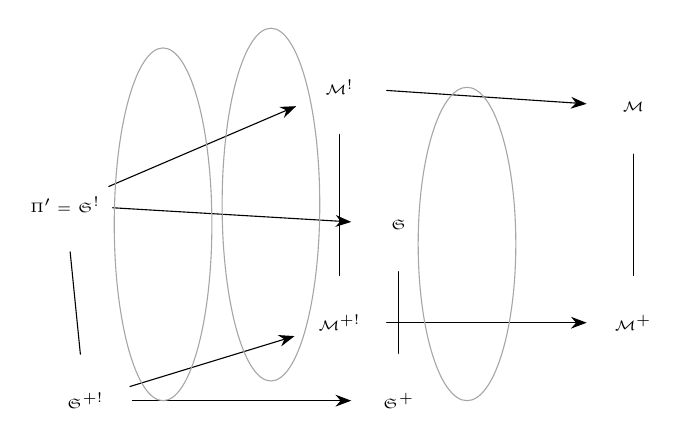
\begin{tikzpicture}[x=1mm,y=1mm,line cap=round,line join=round,font=\scriptsize]
\node[inner sep=1pt] at (16.2,-25.3) {\tiny $\Pi'=\mathfrak S^!$};
\node[inner sep=1pt] at (58.5,-27.8) {\tiny $\mathfrak S$};
\node[inner sep=1pt] at (51,-10.4) {\tiny $\mathcal M^!$};
\node[inner sep=1pt] at (88.3,-12.9) {\tiny $\mathcal M$};
\node[inner sep=1pt] at (51,-40.3) {\tiny $\mathcal M^{+!}$};
\node[inner sep=1pt] at (88.3,-40.3) {\tiny $\mathcal M^+$};
\node[inner sep=1pt] at (18.7,-50.2) {\tiny $\mathfrak S^{+!}$};
\node[inner sep=1pt] at (58.5,-50.2) {\tiny $\mathfrak S^+$};
\draw[-{Stealth[length=2mm]}] (21.7,-23) -- (45.5,-12.8);
\draw[-{Stealth[length=2mm]}] (57,-10.8) -- (82.4,-12.5);
\draw (51,-16.4) -- (51,-34.3);
\draw (88.3,-18.9) -- (88.3,-34.3);
\draw[-{Stealth[length=2mm]}] (57,-40.3) -- (82.4,-40.3);
\draw[-{Stealth[length=2mm]}] (22.2,-25.7) -- (52.5,-27.5);
\draw[-{Stealth[length=2mm]}] (24.7,-50.2) -- (52.5,-50.2);
\draw (16.8,-31.3) -- (18.1,-44.3);
\draw[-{Stealth[length=2mm]}] (24.4,-48.4) -- (45.3,-42);
\draw (58.5,-33.8) -- (58.5,-44.2);
\draw[struck] (28.6,-27.8) ellipse[x radius=6.2, y radius=22.4];
\draw[struck] (42.3,-25.3) ellipse[x radius=6.2, y radius=22.4];
\draw[struck] (67.2,-30.3) ellipse[x radius=6.2, y radius=19.9];
\end{tikzpicture}
\end{document}
